\documentclass[emulatestandardclasses]{scrartcl}
\usepackage{graphicx}
\usepackage{color}
\usepackage[ngerman]{babel}
\usepackage{hyperref}
\usepackage{fullpage}
\usepackage[utf8]{inputenc}
\usepackage{calc} 
\usepackage{enumitem}
\usepackage{titlesec}
\newcommand{\todo}[1]{\textcolor{red}{TODO: #1}\PackageWarning{TODO:}{#1!}}
\date{\vspace{-3ex}}
\begin{document}

\title{
	\includegraphics*[width=0.75\textwidth]{ErstesSem/images/hu_logo.png}\\
	\vspace{24pt}
	Plato's Phaedo}
\subtitle{\vspace{10pt}Proseminar WS 17/18\\
          David Ebrey\\
          Philosophisches Institut I \\ 
          Humboldt Universit"at zu Berlin}
\author{Lennard Wolf\\
        \small{\href{mailto:lennard.wolf@student.hu-berlin.de}{lennard.wolf@student.hu-berlin.de}}}
\maketitle
\begin{abstract}
In this seminar we will carefully work through Plato's Phaedo, which discusses ethical, epistemological, and metaphysical ideas that at the heart of Plato’s philosophy. Topics covered include: causation, the nature of the soul, the problems caused by the body, how inquiry is possible, the proper attitude and methodology for inquiry, why (and in what sense) the forms are distinct from sensible things, and why the best life is spent contemplating the forms. We will also discuss how the literary elements of the dialogue are related to its philosophical ideas.
The seminar will be in English and will assume basic familiarity with Plato's works. Knowledge of Greek is not required, but we will occasionally discuss the Greek, as needed.
\end{abstract}
\newpage

\tableofcontents
%\listoffigures
\newpage


\section{Introduction\\(19.10.17)}

\begin{itemize}
  \item Reading: Phaedo until next week
  \item Should read Laches before!
  \item Ecthyphro would be good 
  \item laches authyphro cooper
  \item Apology!!
  \item every week one page assignment to write what is confusing you?
  \item 15 to 20 pages! during the semester meeting! what is the central question to answer in the paper? how to go about it? hand in draft by March 15!
  \item apology, laches, phaedo 
  \item The early/Socratic dialogues: Laches, Euthyphro, Apology
  \item "`Unfolding Struucture"' of the dialogue: some claims are explained later in the text, but not explicitly!
  \item What is it? $\rightarrow$ "`Form"' 
\end{itemize}


\subsection{Apologie}

\begin{itemize}
  \item Werde anders sprechen als vllt erwartet
  \item Gegen zwei Klagen muss verteidigt werden: 1. alte Beschuldigungen, die schon lange herrschen: er treibe Naturphilosophie und darauf basierende Verleumdungen, er argumentiere ohne Rücksicht auf Wahrheit, 2. neue Klagen, eben erst vorgetragen, er lehre diese Dinge für Geld (Meletos)
  \item Klage: "`Sokrates tut Unrecht und treibt Unnützes, indem er erforscht, was unter der Erde und am Himmel ist, die schwächere Rede zur stärkeren macht, und dies auch unterrichtet."'
  \item Zur Verteidigung will er von altem Vorurteil befreien
  \item Verteidigung: Ich habe nichts dergleichen getan, fragt euch gegenseitig als Zeugen, niemand wird so etwas behaupten (?) $\rightarrow$ aber warum wird dann geklagt und warum spricht niemand dagegen?
  \item Orakel von Delphi: Sokrates ist intelligentester von allen $\rightarrow$ was heißt das?
  \item Geht zu scheinbar klugem Politiker um ihm zu zeigen, er sei nicht so klug wie er denkt, doch das hat ihn nur verhasst gemacht
  \item Beide wissen nichts, doch Unterschied: der andere glaubt etwas zu Wissen, Sokrates nicht
  \item Ich bin darum klüger "`dass ich, was immer ich nicht weiß, auch nicht zu wissen glaube."'
  \item Dieses Unwissen lehrt er, im Namen des Gottes
  \item Du jungen Leute folgen ihm und ahmen ihm nach, die anderen zu prüfen
  \item Die Leute werden zornig und meinen, Sokrates verzöge die Jugend
  \item Daher klagen sie ihn nun an (Ende Verteidigung 1)
  \item Meletos: interessiere sich gar nicht für die Jugend, da er sich nie gefragt hat, wer sie wie bessern könne
  \item Niemand will sich selbst schaden, also kann er die Jugend nicht absichtlich verderben, da ihm sonst Schaden zukommt, also muss er es, wenn er es tut, unabsichtlich tun
  \item Das Gesetz sagt, dass so einem Menschen nur im Privaten auf die Finger gehauen werden soll \emph{schlechtes Argument, damit wäre jeder Täter unschuldig}
  \item Frage: \emph{wie} wird die Jugend verdorben? Klage: Gottlosigkeit und Dämonenglaube
  \item Sokrates zeigt Widerspruch, denn um Dämonendinge zu lehren kann er nicht gottlos sein (Ende Verteidigung 2)
  \item Doch was ihn zu Fall bringen wird sind nicht die Klagen, sondern die Missgunst der Masse
  \item Schämst du dich nicht Dinge zu tun, die dich in Gefahr bringen? - Dann wären auch die Heroen von Troja unwürdig. Die Schande ist doch schlimmer als der Tod!
  \item Die Angst vor dem Tode setzt den Glauben voraus, der Tod sei das schlimmste!
  \item "`Mein Bester, du bist Athener, ein Bürger der größten und durch Bildung und Macht berühmtesten Stadt, und du schämst dich nicht, dich darum zu kümmern, wie du zu möglichst viel Geld und wie du [e] zu Ehre und Ansehen kommst, doch um die Vernunft und die Wahrheit und darum, dass du eine möglichst gute Seele hast, kümmerst und sorgst du dich nicht?"'
  \item Selbst wenn ihr mich freisprecht, ich werde immer dem Gott dienen und mich und die anderen zu Erkenntnis bewegen. Wenn ihr mich tötet schadet ihr euch mehr als mir.
  \item Die Kläger konnten keine Zeugen bringen, und dass Sokrates Geld nähme, dagegen ist seine Armut ein Zeuge
  \item War nie politisch aktiv, denn so ungerecht die Umstände auch sind, sie würden ihn nie dazu geleiten, Dinge gegen Gott zu tun (Scheiben einwerfen)
  \item Sokrates habe nie gelehrt, doch wenn einer zuhören will, so verwehrt er es ihm auch nicht
  \item Ende: Ich werde nicht flehen und bitten und Mitleid erzeugen, dies wäre nicht rechtens. Vielmehr wollte ich informieren und überzeugen.
  \item ---- Ende Erste Rede ----
  \item Stellt Antrag auf Speisung im Prytaneion (wurde für besondere Verdienste gewährt und entspricht nach heutigen Vorstellungen der Verleihung einer Ehrenbürgerwürde)
  \item Denn andere Anträge sind unsinnig. Verbannung würde ihn nur in andere Städte schicken und sich alles im Kreis drehen. 
  \item "`Warum nicht mit dem Fragen aufhören?"' - "`Ich muss Gott folgen. ein Leben ohne Prüfung ist für den Menschen nicht lebenswert."'
  \item Antrag auf Geld: Platon et al als Bürgen
  \item ---- Ende Zweite Rede ----
  \item Lieber mit ehrenvoller Verteidigung zugrundegehen, als mit jammernder am Leben bleiben.
  \item Die Richter meinen ihm zu schaden mit der Strafe, doch ist doch vollkommen unklar, was im Tod wirklich passiert. 
  \item Vielleicht ist der Tod ein ruhiger Schlaf - vielleicht trifft er auf die Heroen im Hades.
  \item Ob der Tod oder das Leben das bessere Los ist, das weiß nur der Gott.
  \item ---- Ende Dritte Rede ----
\end{itemize}

\subsection{Euthyphron}

\begin{itemize}
  \item 
\end{itemize}


\newpage
%\section{"Uber den Professor}
%Matthias Schlo"sberger ist Heisenbergstipendiat der Deutschen Forschungsgemeinschaft
%an der Humboldt Universit"at zu Berlin mit dem Forschungsprojekt "`Die Erfahrung der Realit"at durch Widerstand"'.
%
%\begin{figure}[h]
%	\centering
%	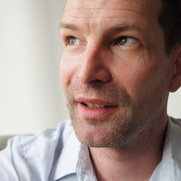
\includegraphics[width=0.3\textwidth]{images/Matthias_Schlossberger.png}
%	\caption{Matthias Schlo"sberger}
%	\label{fig:MS}
%\end{figure}


%\begin{figure}[h]
%	\centering
%	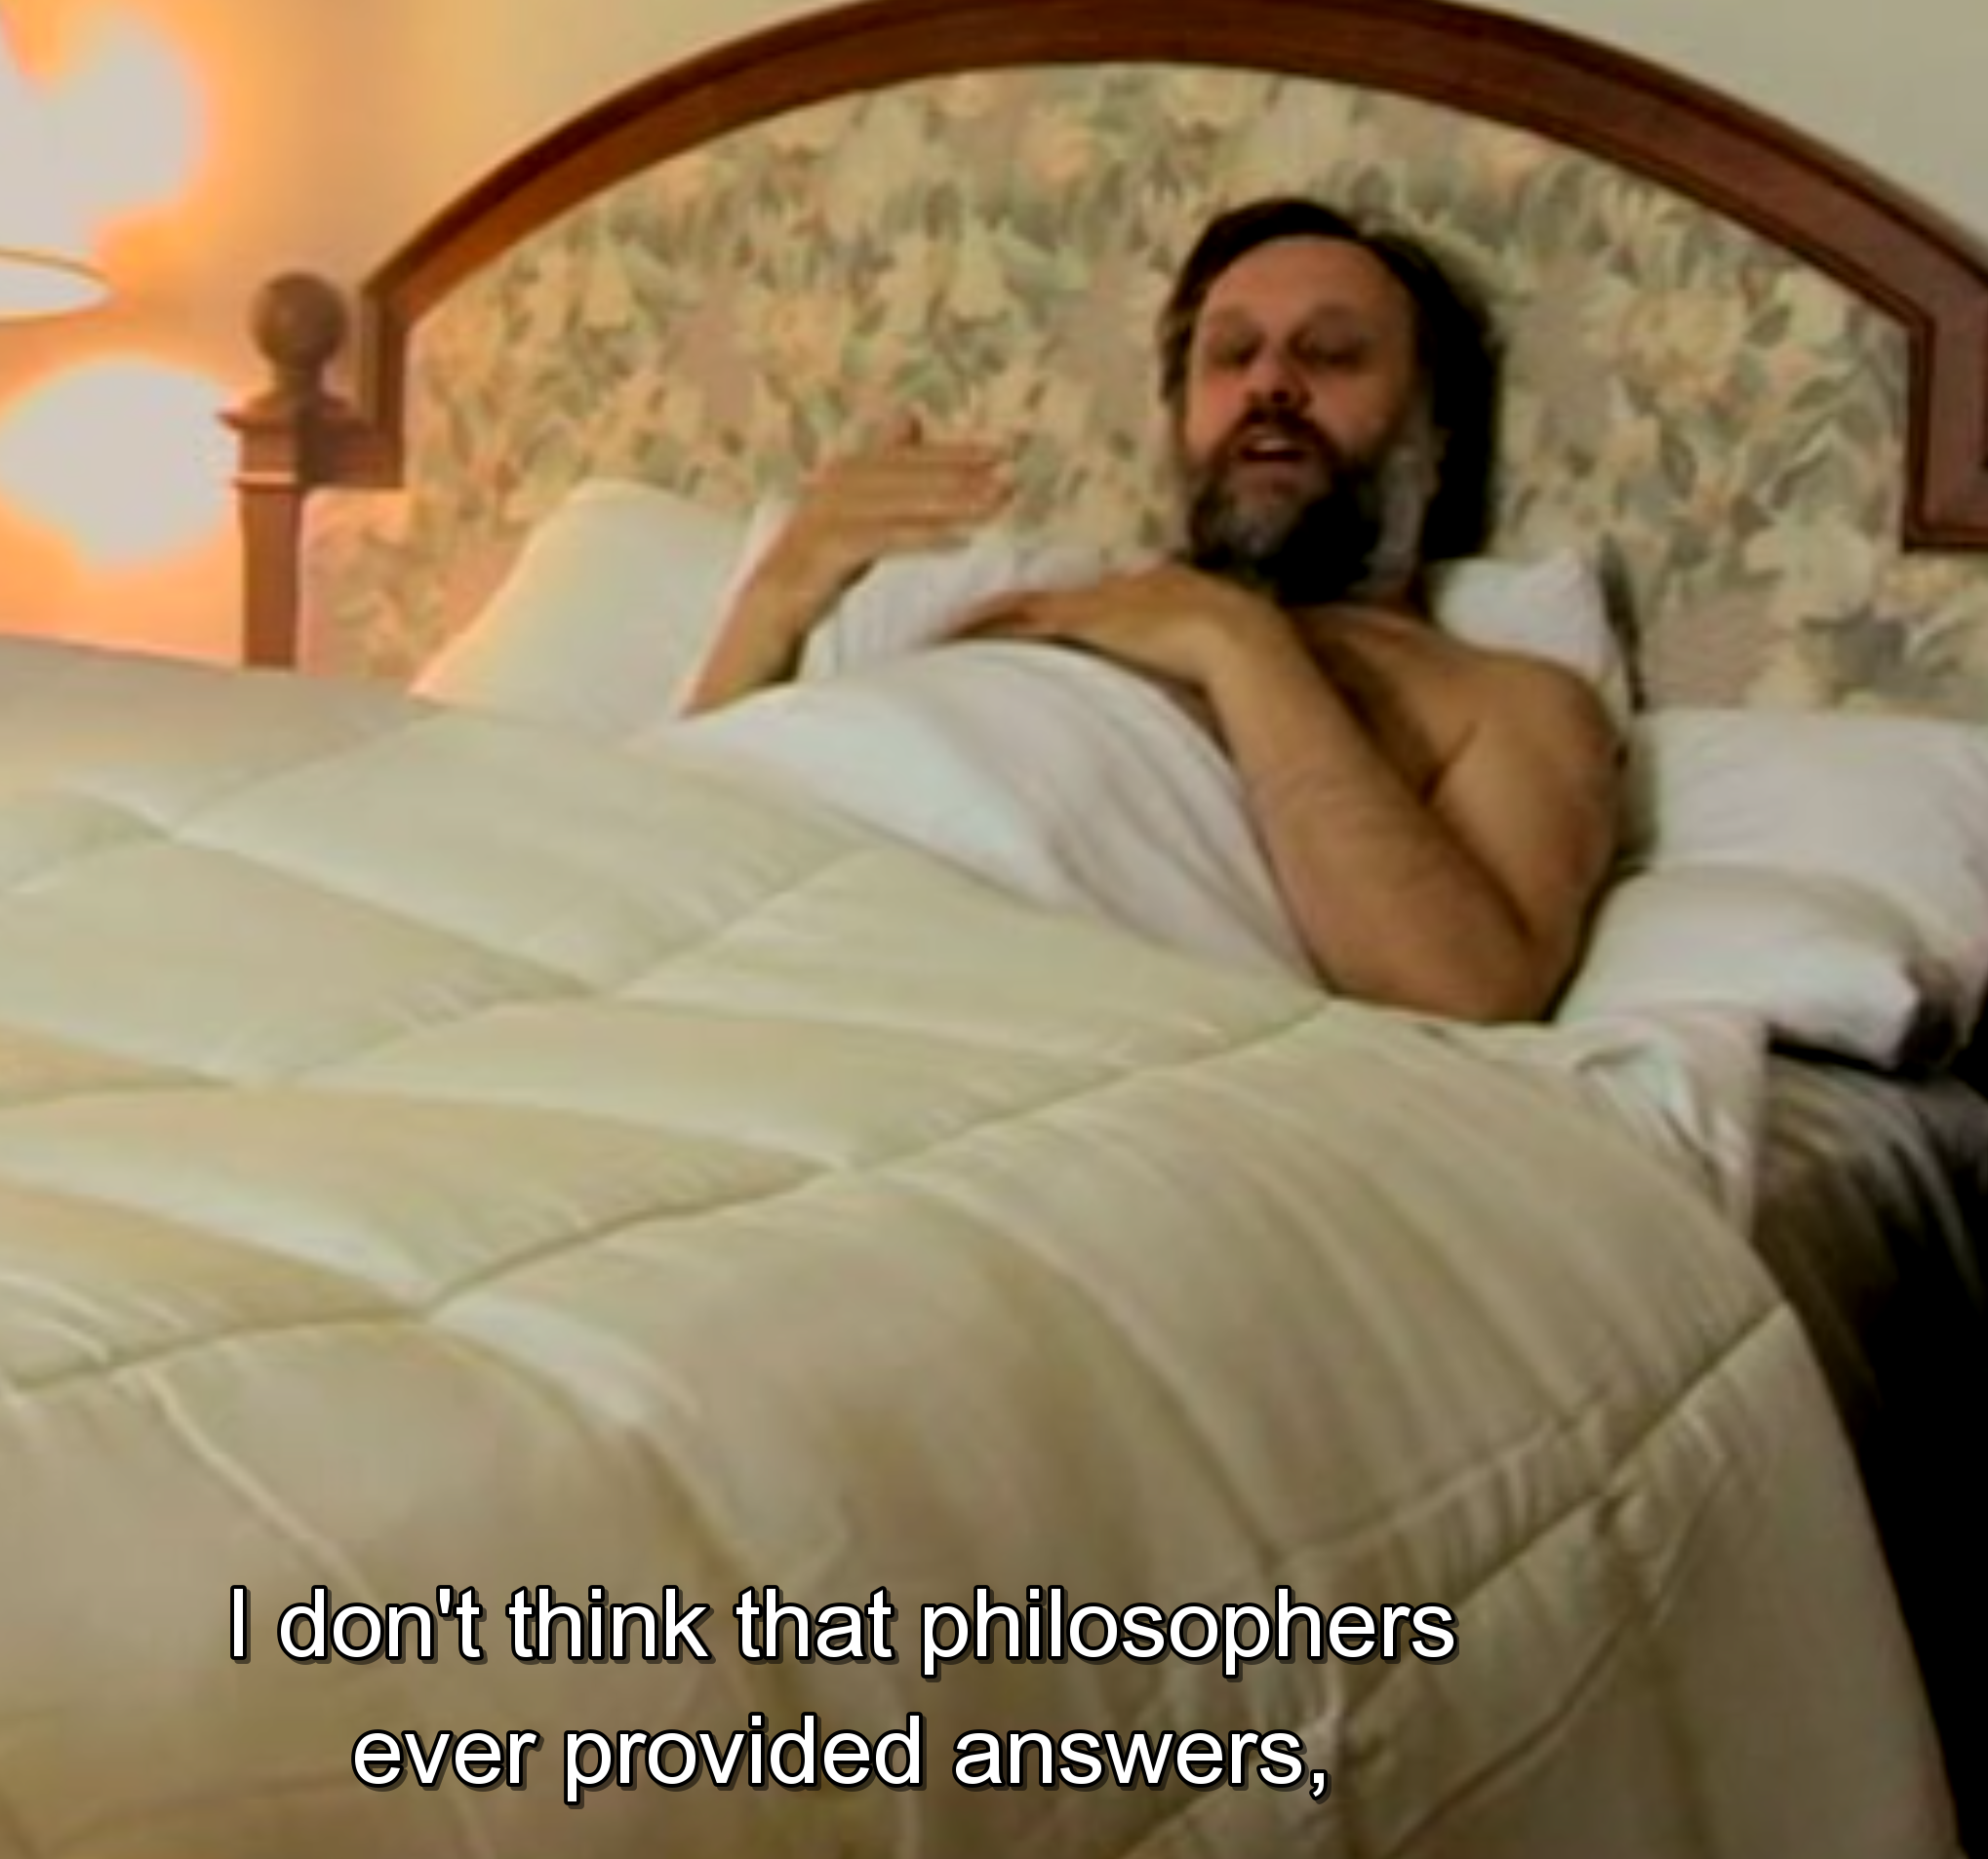
\includegraphics[width=0.5\textwidth]{images/template.png}
%	\caption{Template Bild}
%	\label{fig:template}
%\end{figure}

\end{document}
